\chapter{Organisation}\label{chap:organisation}

\cbstart

\section{Sejlklubben Sundet}

I følgende afsnit beskrives nogle sejlklubbers opbygning, herfra vil der blive konkluderet på en generel opbygning af
disse, og slutteligt hvilke funktioner de forskellige medlemmer har i klubben.

\subsection{Research af klubber}\label{subsec:research}


Sejlklubben Sundet, som ligger i København Ø 2100 på Svaneknoppen 8, har flere både, af forskellig størrelse, som bruges
til undervisning af klubbens elever, såvel som udlån til klubbens medlemmer. Undervisningen foregår i sejlerskolen, med
undervisning om hverdagene. Uddannelsen varer 2 år, og man lærer at sejle både i Drabant 24, og
Gaffelrigger.\fxnote{måske der skal en fodnote ind om hvad de her to ting er?} Man kan i klubben, som nævnt, låne bådene
til sejladser for et mindre beløb, men hvis en af skolens elever er med, er dette gratis
at gøre. Det er dyrere at leje i weekenderne end i hverdagene. I forbindelse med en sæson på sejlerskolen, er man ude
og sejle op til 18 gange typisk fra 18:00-21:00 en gang om ugen. Der sejles desuden kun i maj, juni, august og
september. Når skolen er færdig og man har bestået førerprøven er man if. Sundets reglementer Bådfører, og man får
tildelt sit eget certifikat.

For at en besætning må sejle skal der være minimum én fører med i bådens besætning \fxnote{Husk at definere fører og
muligvis besætning, hvis dette bibeholdes. - Søren, er det fikset nu ? Har beskrevet fører,og besætning siger lidt sig
selv? }. Desuden bestemmes prisen for udlånet bl.a. efter besætning også, idet tilstedeværelsen af en af klubbens elever
gør, at udlånet er gratis.\citep{Sundet}

Sundets hjemmeside givet begrænset mulighed for information på medlemmer, derfor sker håndteringen af medlemmernes
information mm. muligvis på papir, eller ved en lokal computer ved manuelt arbejde, hvilket ifølge oplysninger
\fxnote{Muligvis angive en mere officiel kilde her?} kan resultere i, at det kun bliver gjort engang imellem.\fxnote{Hvad menes
helt konkret her, synes det er en lidt tynd beskrivelse? - Og er det vigtigt ? }

Ved et kig på Sejlklubben Sundets hjemmeside \citep{SundetUdlaan} ses det, at forskellige værktøjer bl.a. en doodle
taget i brug, i et forsøg på at øge brugervenlighed og interaktion mellem deltagere. Det er på nuværende tidspunkt
uvist, hvor vidt disse tiltag har haft den ønskede, gavnlige effekt.

Sejlklubben bestemmer sin ledelse ved generalforsamlinger. Her bliver der også valgt, regnskabsfører, øvrige
bestyrelsesmedlemmer, samt en revisor og revisorsuppleant. Kun æresmedlemmer eller aktive medlemmer over 18 år har
stemmeret ved generalforsamlingen. Stemmeretten udøves ved personligt fremmøde til forsamlingen. Medlemmerne kan senest
seks uger før generalforsamlinger sende forslag til diskussioner, såsom vedtægtsændringer, eksklusioner af medlemmer ol.
Det er altså demokratiske valg der håndterer større beslutninger i klubben.

En anden sejlklub, Aalborg Sejlklub som findes på Skydebanevej 40, Aalborg 9000, ved Marina Fjordparken. Der findes
mindre information på deres hjemmeside, end ved Sundet, men Aalborg Sejlklub har også en sejlerskole, som indeholder en
praktisk prøve, \fxnote{Jeg har sendt en mail for at høre hvad formålet med skolen er, for man sit førerbevis ? - Det
står ikke angivet på deres hjemmeside.} Aalborg Sejlklub administreres på samme lign. måde som Sundet gør. De har en
Ordinær Generalforsamling, hvor der stemmes for hvem der skal have de bestyrende roller. I Aalborg Sejlklub findes også en næstformand. Ved Generalforsamlingen har alle medlemmer over 18
år stemmeret, og den udøves på samme måde som ved Sundet, i form af personligt fremmøde.\citep{AalborgSejlklub}

En tredje klub, Bådklubben Valby, har stor set samme fordeling af medlemmer, og deres funktioner. De holder Generalforsamling, hvor bestyrelsesmedlemmer vælges. Bådklubben har ikke en skole på samme måde, men de har dog stadig kurser således man kan opnå sit duelighedsbevis hos dem.\citep{BaadklubbenValby}


\subsection{Konklusion af Organisationsanalyse}

De 3 klubber der er undersøgt har mange ting til fælles i deres organisation, og følgende model er blevet lavet af bådklubbers organisation. 

\begin{figure}[htbp]
  \centering
  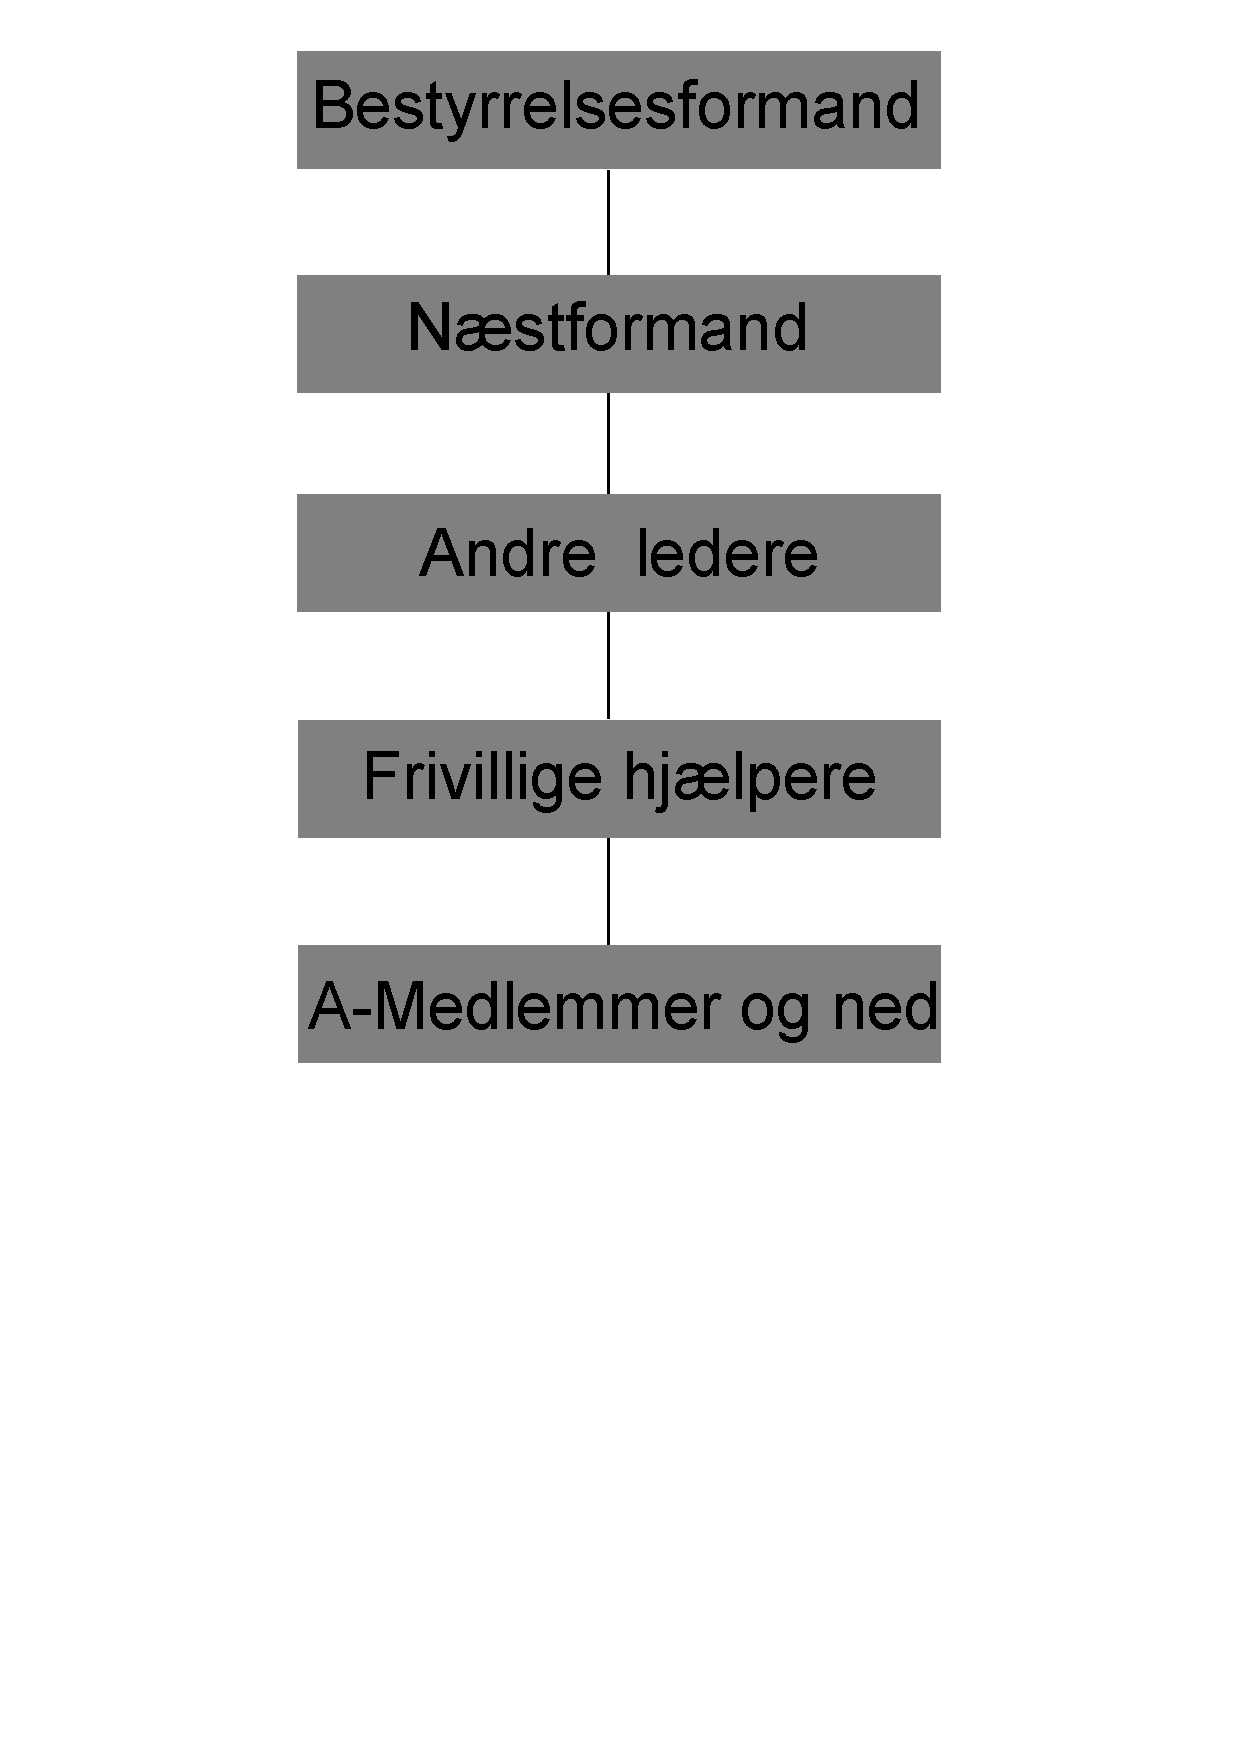
\includegraphics[width=0.5\textwidth]{images/organisation/baadOrganisation.pdf}
  \caption[Bådklubs organisation]{Illustration af elementerne i en bådklubs organisation.}
  \label{fig:bådklub-organisation}
\end{figure}

Modellen viser at øverst findes Bestyrelsesformanden, som skal sørge for at klubben kører som den skal, der kan være en næstformand, som hjælper til hvis opgaverne er for store for formanden. De andre ledere, er sekretærene, de økonomisk styrende, og underviserne til skolerne, disse er dog betalte. Derefter er der de frivillige hjælpere, som kan have samme funktioner som de førnævnte ledere. Man kan forestille sig de betalte ledere har mere ansvar end de frivillige. Nederst er de normale medlemmer, som kun bruger klubbens faciliteter, og hvor nogle af dem har stemmeret til generalforsamlingerne.

Medlemmerne betaler kontingenter for at være medlem, og for at kunne benytte sig af klubbens faciliteter. Det er herudover meget forskelligt fra klub til klub, hvilke frynsegoder der er ved at hjælpe til i klubben.

Efter denne undersøgelse er der altså dannet en forståelse af hvordan bådklubberne er opbygget, og ud fra denne information, kan man danne et overblik over hvilke funktioner en bådklub ville kunne drage nytte af i forbindelse med et IT-system.

\fxnote{Dette er blot et foreløbt udkast til funktioner, det kan være der skal lidt mere information til for at kunne drage disse konklusioner. }

\begin{itemize}
	\item Medlemmer skal kunne leje både, og angive hvem af klubbens medlemmer besætningen består af.
	\item Medlemmer bør kunne holde øje med lektioner og være i stand til at melde sig på lektionerne.
	\item Der bør være en liste over medlemmer, så medlemmerne indbyrdes kan tage kontakt til hinanden.
	\item Der bør være et kontaktmedium så medlemmerne kan kontakte hinanden, eller spørge på et forum om diverse emner.
	\item Det bør være muligt for formanden let at dele meddelelser med klubbens medlemmer. 
	\item Medlemmerne bør være i stand til at betale for deres kontingenter over nettet, for at nedsætte det manuelle arbejde fra klubbens frivillige.
\end{itemize}
\cbend
